\section{Testläufe mit initialer Konfiguration}
Ziel dieser ersten Testläufe war es, herauszufinden, inwieweit das Fehlerziel 
mit den gewählten Parametern erreicht werden kann. Es wurden dabei jeweils 10 
Testläufe mit identischen Parametern durchgeführt, um "`Zufallstreffer"' 
(Gewichts- und Biaswerte werden bei Initialisierung des Netzes zufällig 
vergeben) auszuschließen. Tabelle \ref{tbl:21-5-3-ergebnisse} zeigt einen
Überblick über diesen Testlauf.

\begin{table}
	\sffamily
	\centering
	\footnotesize
	\begin{tabular}{Nllc}
		\toprule
		\multicolumn{1}{@{}N}{Nr.} &
		\multicolumn{1}{V{3.5em}@{}}{Epoche} &
		\multicolumn{1}{V{3.5em}@{}}{MSE} &
		\multicolumn{1}{V{5em}@{}}{Ziel erreicht} \\
		\midrule\addlinespace

		1 & 781 & 3.239147e-003 & --- \\ \cmidrule(rl){1-4}
		2 & 268 & 3.237180e-003 & --- \\ \cmidrule(rl){1-4}
		3 & 2000 & 1.390480e-003 & --- \\ \cmidrule(rl){1-4}
		4 & 887 & 2.027749e-002 & --- \\ \cmidrule(rl){1-4}
		5 & 2000 & 1.708763e-003 & --- \\ \cmidrule(rl){1-4}
		6 & 664 & 1.756893e-002 & --- \\ \cmidrule(rl){1-4}
		7 & 1610 & 9.666874e-005 & $\checkmark$ \\ \cmidrule(rl){1-4}
		8 & 655 & 2.314696e-003 & --- \\ \cmidrule(rl){1-4}
		9 & 1737 & 1.851531e-003 & --- \\ \cmidrule(rl){1-4}
		10 & 338 & 3.238135e-003 & --- \\ 

		\addlinespace\bottomrule
		\end{tabular}
	\caption{Ergebnisse der Testreihe mit 21-5-3 Netz}
	\label{tbl:21-5-3-ergebnisse}
\end{table}

Lediglich ein Testlauf erreichte hier das Fehlerziel - die anderen brachen bei 
Erreichen der maximalen Epochenanzahl bzw. des minimalen Gradienten ab. 
Abbildung \ref{fig:plot-runs-1} zeigt beispielhaft den Verlauf der Performance 
(also des MSE) für Testlauf Nr. 1, Abbildung \ref{fig:plot-runs-7} zeigt den 
erfolgreichen Testlauf Nr. 7.

\begin{figure}
  \centering
  \subfloat[Testlauf Nr. 1: minimaler Gradient erreicht]{
    \label{fig:plot-runs-1}
    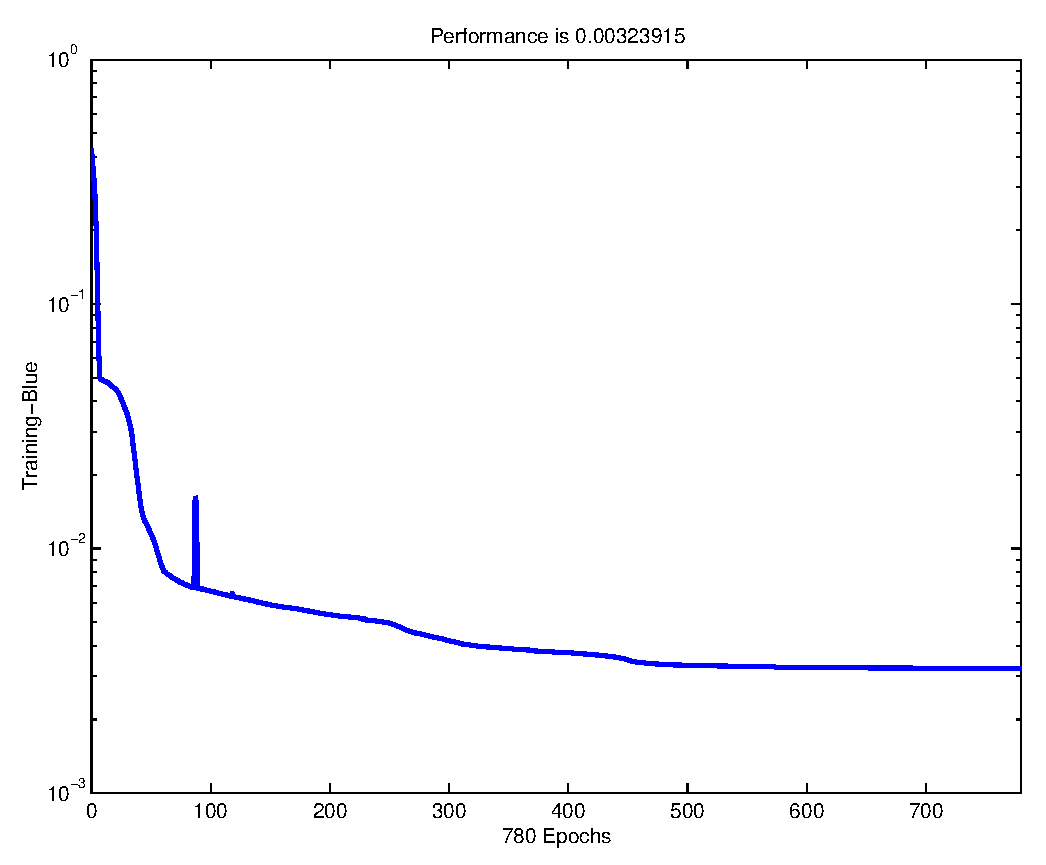
\includegraphics[width=0.45\textwidth]{../images/plots/21-5-3/21-5-3_1}
  }
  \subfloat[Testlauf Nr. 7: erfolgreich]{
    \label{fig:plot-runs-7}
    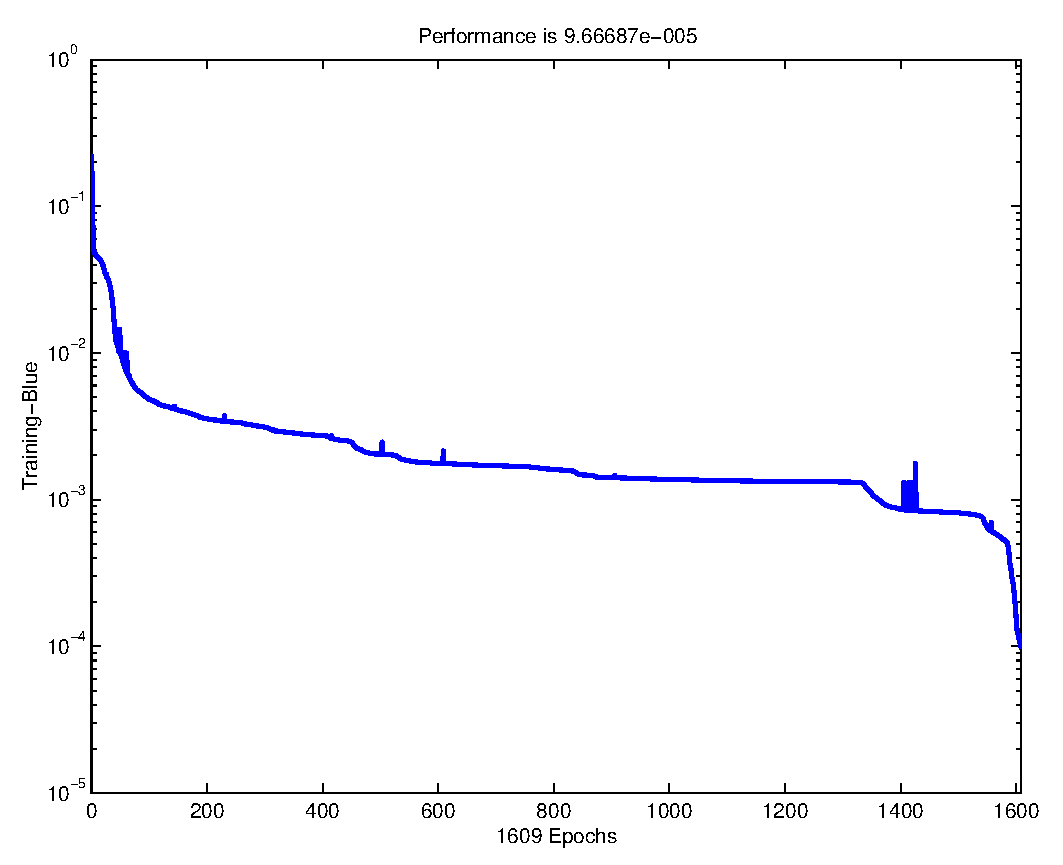
\includegraphics[width=0.45\textwidth]{../images/plots/21-5-3/21-5-3_7}
  }
  \caption{Verlauf der Performance zweier Testläufe}
  \label{fig:plot-runs}
\end{figure}

\section{Variation der Netzkonfiguration}
Wie im vorherigen Abschnitt zu sehen, erreichte das Netz mit nur 5 Neuronen in 
einer verdeckten Schicht das vorgegebene Fehlerziel (MSE) von $1 \cdot 10^{-4}$
lediglich in einem der Testläufe. Daher werden nun in einem ersten Schritt die
Anzahl der Neuronen in der verdeckten Schicht erhöht. Tabelle
\ref{tbl:var-neuronen} zeigt die Ergebnisse für diesen Versuch; in der letzten
Spalte ist aufgeführt, wie viele der 10 Testläufe das Fehlerziel erreicht haben. 

\begin{table}
	\sffamily
	\centering
	\footnotesize
	\begin{tabular}{lllc}
		\toprule
		\multicolumn{1}{V{7em}@{}}{Neuronen 1. verdeckte Schicht} &
		\multicolumn{1}{V{7em}@{}}{Epoche Durchschnitt} &
		\multicolumn{1}{V{7em}@{}}{MSE Durchschnitt} &
		\multicolumn{1}{V{5em}@{}}{Ziel erreicht} \\
		\midrule\addlinespace

		10 & 690 & 1.129535e-003 & 2/10 \\ \cmidrule(rl){1-4}
		15 & 473 & 1.222659e-003 & 2/10 \\ \cmidrule(rl){1-4}
		20 & 463 & 9.913476e-004 & 2/10 \\ \cmidrule(rl){1-4}
		25 & 391 & 8.526345e-004 & 2/10 \\ \cmidrule(rl){1-4}
		30 & 382 & 6.968107e-004 & 5/10 \\ \cmidrule(rl){1-4}
		35 & 382 & 6.957020e-004 & 5/10 \\ \cmidrule(rl){1-4}
		40 & 379 & 9.908886e-004 & 2/10 \\ \cmidrule(rl){1-4}
		45 & 380 & 1.195249e-003 & 4/10 \\ \cmidrule(rl){1-4}
		50 & 315 & 1.176323e-003 & 2/10 \\ 

		\addlinespace\bottomrule
		\end{tabular}
	\caption{Ergebnisse der Testreihe mit variierender Neuronenzahl}
	\label{tbl:var-neuronen}
\end{table}

Wie sich zeigt, wird das Fehlerziel in dem Netz mit \emph{einer} verdeckten Schicht 
maximal in 50\% der Testläufe erreicht. Es wird nun in einem weiteren Versuch 
mit einem Netz mit \emph{zwei} verdeckten Schichten gearbeitet. Auch hier wird wieder wie 
zuvor die Anzahl der Neuronen variiert und mit jeweils 10 Testläufen 
gearbeitet. Es werden hier nur die vielversprechendsten Kombinationen getestet;
Tabelle \ref{tbl:var-schichten} zeigt die Ergebnisse.

\begin{table}
	\sffamily
	\centering
	\footnotesize
	\begin{tabular}{llllc}
		\toprule
		\multicolumn{1}{V{7em}@{}}{Neuronen 1. verdeckte Schicht} &
		\multicolumn{1}{V{7em}@{}}{Neuronen 2. verdeckte Schicht} &
		\multicolumn{1}{V{7em}@{}}{Epoche Durchschnitt} &
		\multicolumn{1}{V{7em}@{}}{MSE Durchschnitt} &
		\multicolumn{1}{V{5em}@{}}{Ziel erreicht} \\
		\midrule\addlinespace

		10 & 10 & 328 & 1.581422e-003 & 1/10 \\ \cmidrule(rl){1-5}
		15 & 15 & 327 & 5.940588e-004 & 4/10 \\ \cmidrule(rl){1-5}
		30 & 30 & 210 & 4.081598e-004 & 5/10 \\ \cmidrule(rl){1-5}
		35 & 35 & 215 & 4.459380e-004 & 4/10 \\ \cmidrule(rl){1-5}
		45 & 45 & 174 & 3.408588e-004 & 7/10 \\

		\addlinespace\bottomrule
		\end{tabular}
	\caption{Ergebnisse der Testreihe mit zwei verdeckten Schichten}
	\label{tbl:var-schichten}
\end{table}

Wie man den Testläufen entnehmen kann, scheint eine Netztopologie 21-45-45-3 am
besten mit dieser Auswahl von Trainigsdaten trainierbar. Daher wird für die
folgenden Simulationsversuche zunächst auf diese Konfiguration zurückgegriffen.

\section{Simulation des Netzes mit ermittelter Konfiguration}
Im ersten Versuch wird hier das Netz mit den verbleibenden Datensätzen 
simuliert, die nicht für das Training verwendet wurden. Dazu wird der folgende
Funktionsaufruf verwendet:

\begin{lstlisting}[numbers=none]
[ySim, pf, af, eSim, perf] = sim(net, simulationData');
\end{lstlisting}

Dabei wird zum einen das trainierte Netz \texttt{net} sowie die zur Simulation
zu verwendenden Daten übergeben. Die Simulation mit einem erfolgreich
trainierten Netz ergab die folgenden Ergebnise:

\begin{description}
  \item[Fehler Klasse 1:] 36/149, d.h. 75,84\% korrekt erkannt.
  \item[Fehler Klasse 2:] 68/331, d.h. 79,46\% korrekt erkannt.
  \item[Fehler Klasse 3:] 55/5999, d.h. 99,10\% korrekt erkannt.
  \item[Gesamtfehler:] 159/6479, d.h. 97,55\% korrekt erkannt.
\end{description}

Wie man sieht, wird in den Klassen 1 und 2 eine weitaus niedrigere 
Klassifikationsgüte erreicht als in Klasse 3. Dies ist auf die geringe Anzahl 
der Trainingsdaten zurückzuführen. Insgesamt erreichte das Netz mit 97,67\% 
jedoch schon ein recht gutes Ergebnis. Um die Generalisierungsfähigkeit des 
Netzes weiter zu steigern, wird nun versucht, die Anzahl der Trainingsdaten zu 
erhöhen. Es werden nicht mehr 10, sondern 50\% der Datensätze für das Training 
verwendet:

\begin{description}
  \item[Fehler Klasse 1:] 21/83, d.h. 74,70\% korrekt erkannt.
  \item[Fehler Klasse 2:] 22/184, d.h. 88,04\% korrekt erkannt.
  \item[Fehler Klasse 3:] 19/3333, d.h. 99,43\% korrekt erkannt.
  \item[Gesamtfehler:] 58/3600, d.h. 98,23\% korrekt erkannt.
\end{description}

Wie man sieht, kann die Klassifikationsgüte insgesamt durch die Erhöhung der
Anzahl der Trainingsdaten leicht verbessert werden. 

\section{Fazit}
Wie die vorangegangenen Versuche gezeigt haben, ist ein künstliches neuronales 
Netz eine fragiles Gebilde, welches von vielen Einflussfaktoren wie z.B. der Anzahl 
und Auswahl der Trainings- und Simulationsdaten beeinflusst wird. Auch die
Bestimmung der "`optimalen"' Netzkonfiguration ist nicht wirklich eindeutig,
sondern wurde hier hauptsächlich durch Testläufe und Intuition bestimmt. 

Insgesamt konnten im besten Fall ca. 98\% der Datensätze korrekt zugeordnet 
werden. Allerdings bleibt die Klassifikationsgüte für die Klassen 1 und 2 recht 
gering, was auf die relativ kleine Anzahl an zur Verfügung stehenden 
Datensätzen zurückzuführen ist. Für die Klassifikation in 
Schilddrüsenüberfunktion bzw. -unterfunktion ist das künstliche neuronale Netz 
also nur bedingt zu gebrauchen - bei der Entscheidung jedoch, ob ein Patient 
\emph{keine} Fehlfunktion hat, erzielt das Netz recht zuverlässige Ergebnisse.
